\runningheader{Introduksjon numerisk integrasjon og derivasjon}{}{Side \thepage\ av \numpages}

\item[] I deloppgaven \ref{oppg:a})-\ref{oppg:e}) skal du jobbe med følgende signal
\begin{equation}
  \label{eq:u}
 \boxed{ u(t) = 2 {\cdot} t^{2} }
\end{equation}
Basert på det diskret signalet $u_{k}$ gjeldende ved
tidspunktene  $t_{k}$ skal 
du numerisk integrere $u_{k}$ og beregne
{\color{blue}\fbox{$y_{k}$}}  
som en tilnæring til operasjonen
\begin{equation}
  y(t)=\int_{0}^{t}u(\tau)d\tau + y(0) \quad \text{gitt } y(0){=}0   \label{eq:y}
\end{equation}
Videre  skal du numerisk derivere  $u_{k}$ for å beregne
{\color{red}\fbox{$v_{k}$}} som en tilnærming til
\begin{equation}
  \label{eq:v}
  v(t) = \frac{d}{dt}u(t)
\end{equation}

Fra matematikken vet du at de analytiske uttrykkene for $y(t)$ og
$v(t)$ er
\begin{equation}
  \label{eq:9}
  {\color{blue}\boxed{y(t) = \frac{2}{3} {\cdot}t^{3}} }
\end{equation}

\begin{equation}
          {\color{red}\boxed{v(t) = 4{\cdot}t}}   \label{eq:9a}
\end{equation}

Disse skal du benytte som ``fasit'' i noen av oppgavene
slik at du visuelt kan sammenligne  med de numeriske beregningene av  
{\color{red}\fbox{$v_{k}$}} og {\color{blue}\fbox{$y_{k}$}}.
Bruken av {\color{red}\fbox{rød}} og {\color{blue}\fbox{blå}} farger
brukes til å skille mellom henholdsvis derivering og integrering.

\newpage

\runningheader{Oppgave a), frivillig}{}{Side \thepage\ av \numpages}

% ********************************************************
% oppgave a) 
% ********************************************************  
\item
  {\bf Numerisk integrasjon og derivasjon i Simulink}
\label{oppg:a}

  
\begin{itemize}
\item Ta utgangspunkt i Simulinkmodellen i skallfilen
  \fbox{\tt oving3\_a\_m\_skallfil.slx}  vist i figur~\ref{fig:1a_dump},
    og implementer ligning~\eqref{eq:u} og de to analytiske løsningene i
    ligning~\eqref{eq:9} og 
    \eqref{eq:9a} i hvert sitt tilhørende subsystem. Bruk
    blokkene \fbox{\tt Clock}, \fbox{\tt Math Function}  hvor du velger \fbox{\tt
      pow} fra rullegardinmenyen,   samt  \fbox{\tt  Product}
    for å lage disse signalene.  {\color{black}Ta med skjermdump av
      de 3 delmodellene i innleveringen.} 
    \begin{figure}[H]
      \centering
      \hspace*{0mm}\scalebox{0.85}{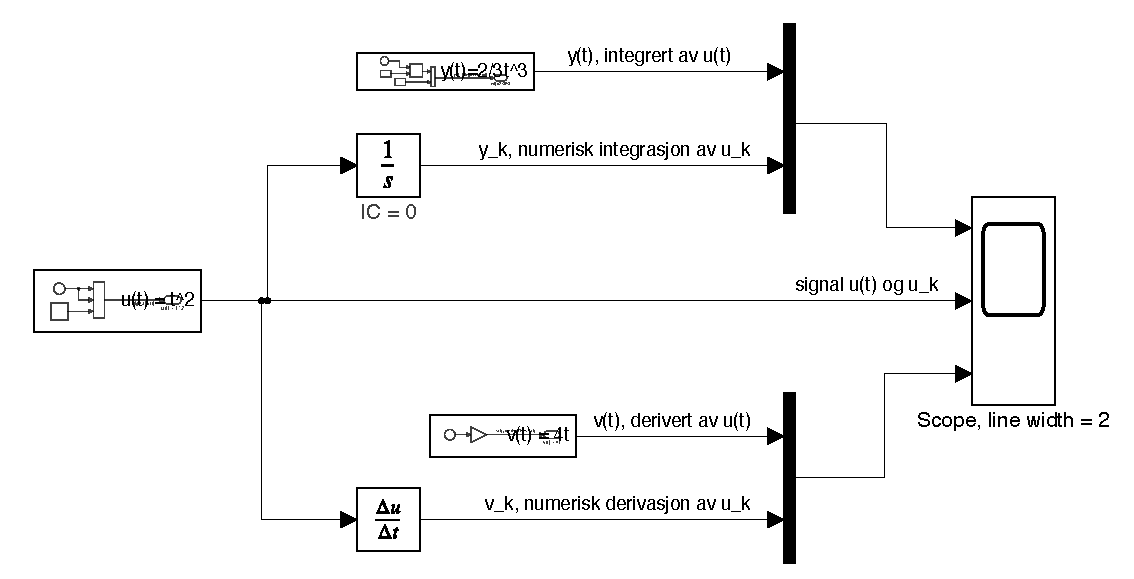
\includegraphics{3a_modell.pdf}}
      \caption{Simulinkmodell hvor ligningene~\eqref{eq:u}, \eqref{eq:9} og 
    \eqref{eq:9a} er implementert i hvert sitt subsystem. }
      \label{fig:1a_dump}
    \end{figure}

    For å sammenligne analytiske og numeriske resultat 
    velger vi å bruke tidspunkt $t{=}2$~sekund. De 
    analytiske verdiene ved dette tidspunktet finner vi fra ligningene~\eqref{eq:9}
    og \eqref{eq:9a} som
    \begin{equation}
      \label{eq:92}
      {\color{blue}{y(2) = \frac{2}{3} {\cdot}2^{3}=5.333}}       
    \end{equation}
    \begin{equation}
      {\color{red}{v(2)  = 4{\cdot}2 = 8}}  \label{eq:9a2}       
    \end{equation}

    For å lese av de  tilsvarende verdiene {\color{blue}\fbox{$y_{k}$}} og
      {\color{red}\fbox{$v_{k}$}} ved $t_{k}{=}2$ sekund i scopet, er
      scopet i skallfilen klargjort med  kurveavlesingsverktøyet
      hentet fra\\ \fbox{\tt Tools -> Measurements -> Cursor
        Measurements}.\\

      Det er  huket av for  \fbox{\tt Snap to data},
      men du må selv velge hvillket signal du skal lese av (i
      skallfilen er  begge avlesningene på $u_{k}$).
      I skallfilen har vi lagt  på markør på kurvene for å fremheve
      beregningstids\-punktene.

      \newpage
\item Spesifiser {\it Eulers forovermetode} ({\tt ode1}) med
  steglengde lik $T_{s}{=}0.4$ sekund, simuler modellen i 3 sekund og
  vis at du får følgende respons
  \begin{figure}[H]
    \centering
    \hspace*{10mm}\scalebox{0.5}{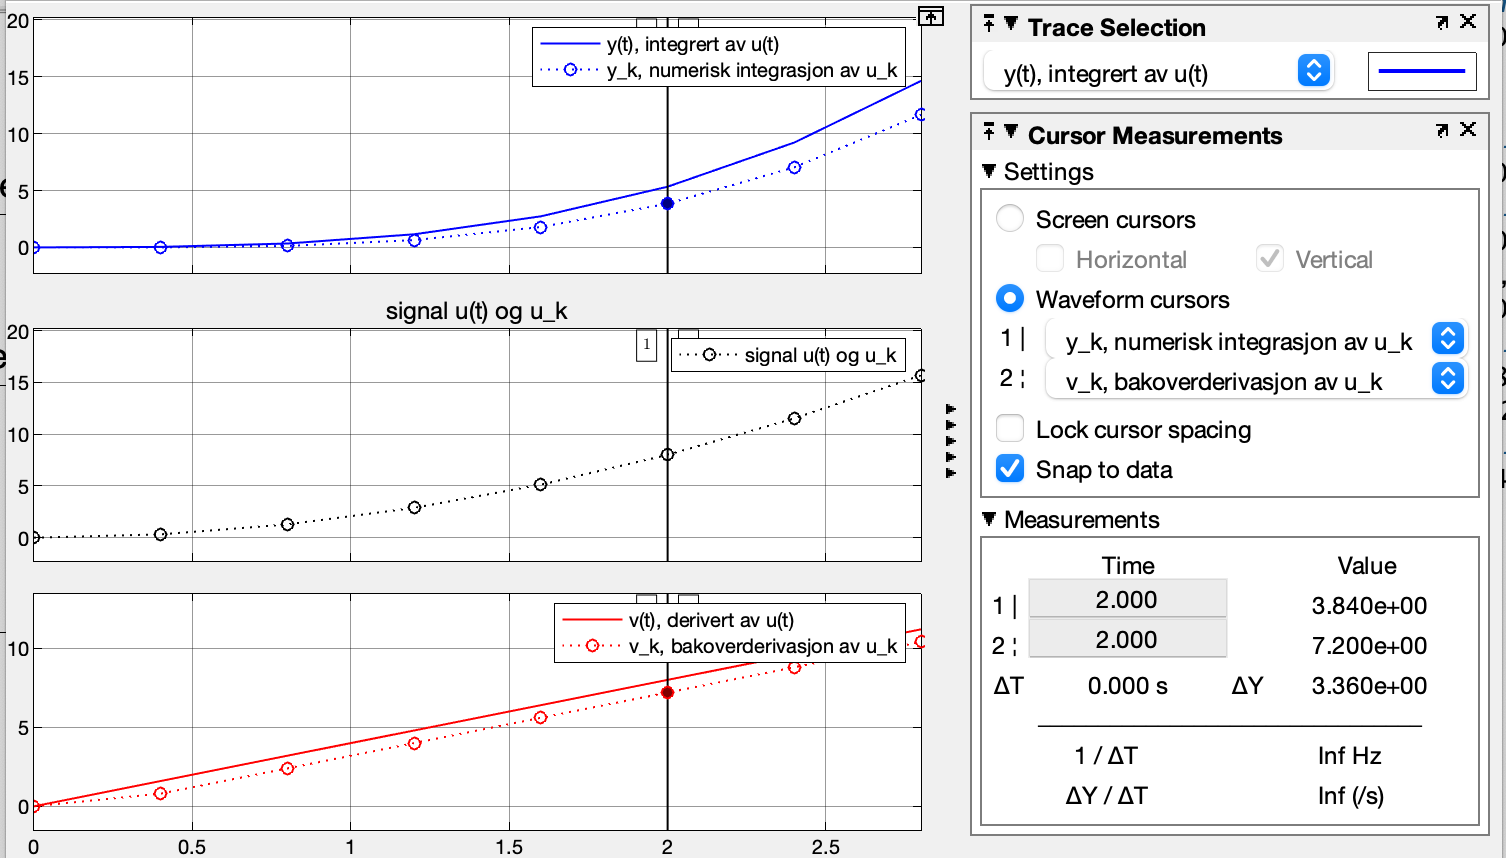
\includegraphics{oppg3a_1.png}}
    \caption{Simuleringsresultat }
    \label{fig:oppg3_1}
  \end{figure}
  
  Ta med din egen respons inkludert avlesingene i innleveringen, og
  vis som over at de avleste verdiene ved $t_{k}{=}2$ sekund er
  \begin{equation}
    {\color{blue}{y_{k}=3.840}}  
  \end{equation}
  \begin{equation}
  {\color{red}{v_{k}=7.2}}   
  \end{equation}
  
      

  \item 
    Spesfiser deretter {\it Eulers bakovermetode} ({\tt ode1be}) med
    samme steglengde og simuler på
    ny. Avles {\color{blue}\fbox{$y_{k}$}} og
    {\color{red}\fbox{$v_{k}$}}  ved samme tidspunkt.
    Ta med din egen respons inkludert avlesingene i innleveringen.

    Gi en forklaring på endringen i den avleste verdien for
    {\color{blue}\fbox{$y_{k}$}}. Gi også en forklaring på hvorfor 
    {\color{red}\fbox{$v_{k}$}} er uendret.


  \item 
    Spesfiser deretter {\it Heuns metode} ({\tt ode2}) som tilsvarer
    {\it trapesmetoden},  og simuler på
    ny. Avles igjen {\color{blue}\fbox{$y_{k}$}} og
      {\color{red}\fbox{$v_{k}$}}  ved samme tidspunkt.
    Ta med din egen respons inkludert avlesingene i innleveringen.

    Gi også her en forklaring på endringen i den avleste verdien for
    {\color{blue}\fbox{$y_{k}$}}. 

\end{itemize}
